
%http://randyridenour.net/2016/04/11/venn-diagrams-with-latex-and-tikz/

\def\sub{(0,0) circle (1.5cm)}
\def\mid{(-60:2cm) circle (1.5cm)}
\def\pred{(0:2cm) circle (1.5cm)}

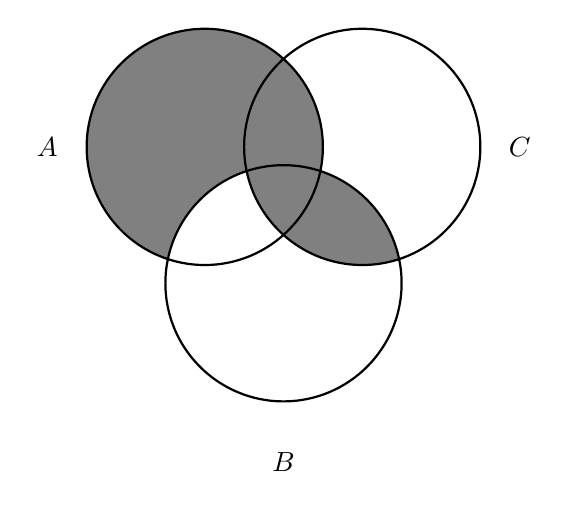
\begin{tikzpicture}[thick]

\begin{scope}
    \draw (-2,-0) node {$A$};
    \draw (1,-4) node {$B$};
    \draw (4,0) node {$C$};

\begin{scope}[even odd rule]% Shade S without M
        \clip \mid (-1.5,-1.5) rectangle (1.5,1.5);
        \fill[gray] \sub;
        \end{scope}

\begin{scope} %Shade intersection of M and P
  \clip \pred;
  \fill[gray] \mid;
\end{scope}

\draw \sub;
\draw \pred;
\draw \mid;
\end{scope}

\end{tikzpicture}